\chapter{Results}\label{chap:res}

\section{Contiguous fill method results}

The following results were generated by using \verb+entropy_cont_fill+\footnote{section \ref{sec:ent_imp}} method.

\begin{figure}[H]
\begin{center}
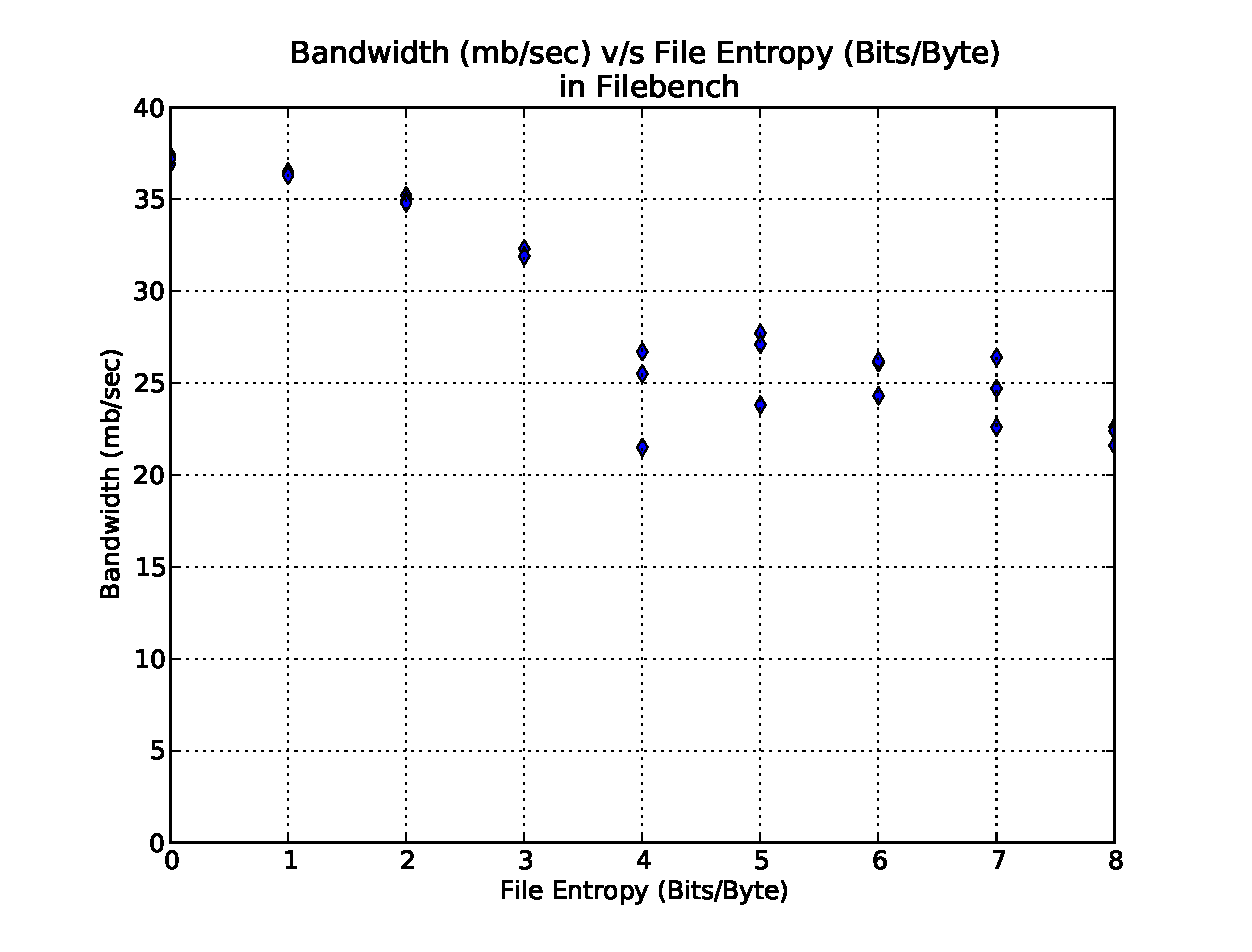
\includegraphics[scale=.55]{../results/set1/write_bw_all.eps}
\caption{The bandwidth of all the write runs}
\label{fig:wb}
\end{center}
\end{figure}

\begin{figure}[H]
\begin{center}
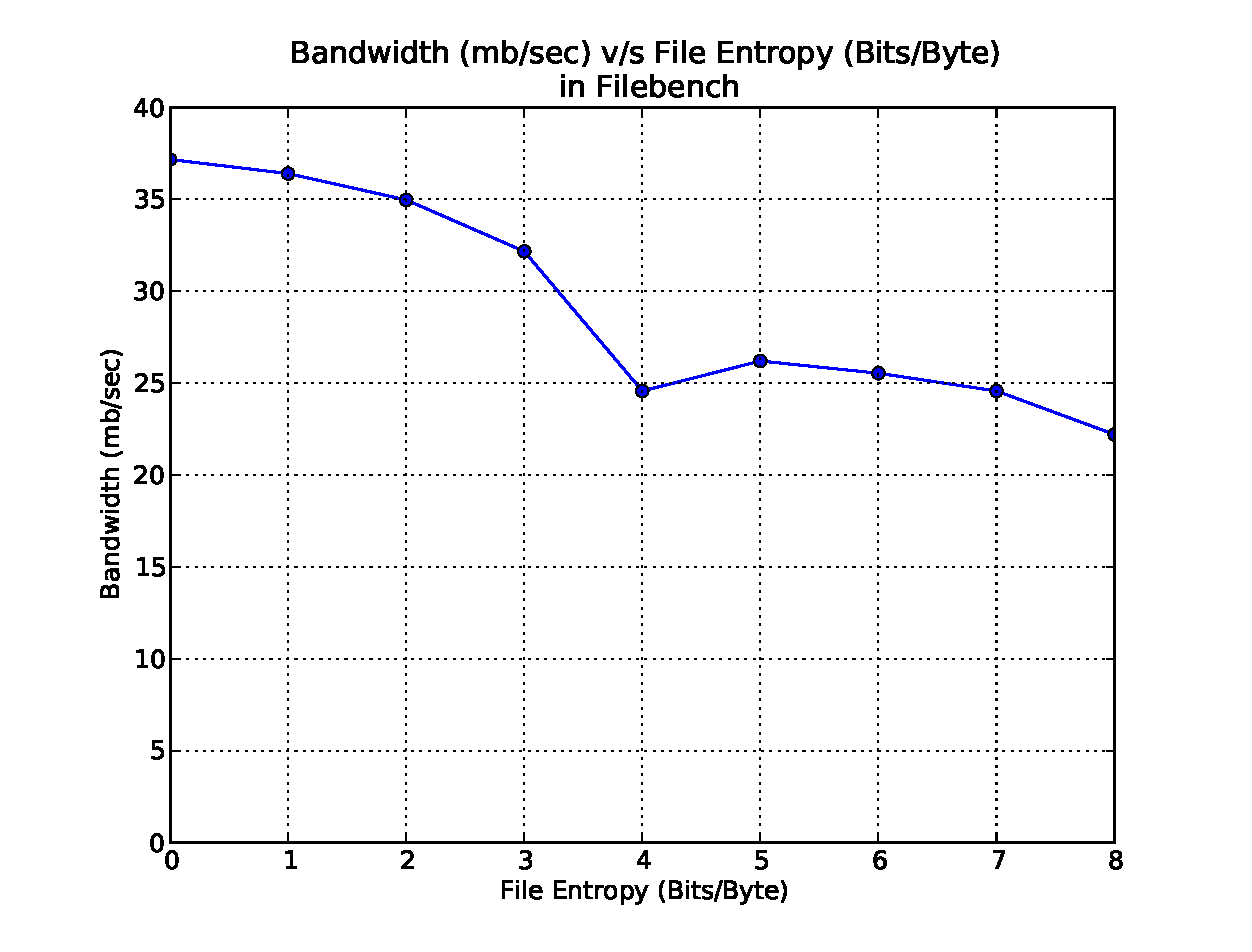
\includegraphics[scale=.55]{../results/set1/write_bw_avg.eps}
\caption{The average bandwidth over all the different write runs}
\label{fig:wbavg}
\end{center}
\end{figure}
\paragraph{}
Figure \ref{fig:wb} and \ref{fig:wbavg} show that bandwidth of the write operation is decreasing as the entropy increased. The larger the entropy the more effort that SDFS spend to deduplicate the files. Figure \ref{fig:wb} shows all values of bandwidth collected from 27 runs. The deviation is small and acceptable. To present all the runs on one plot the average of all the runs for each entropy is calculated and presented in figure \ref{fig:wbavg}.

\begin{figure}[H]
\begin{center}
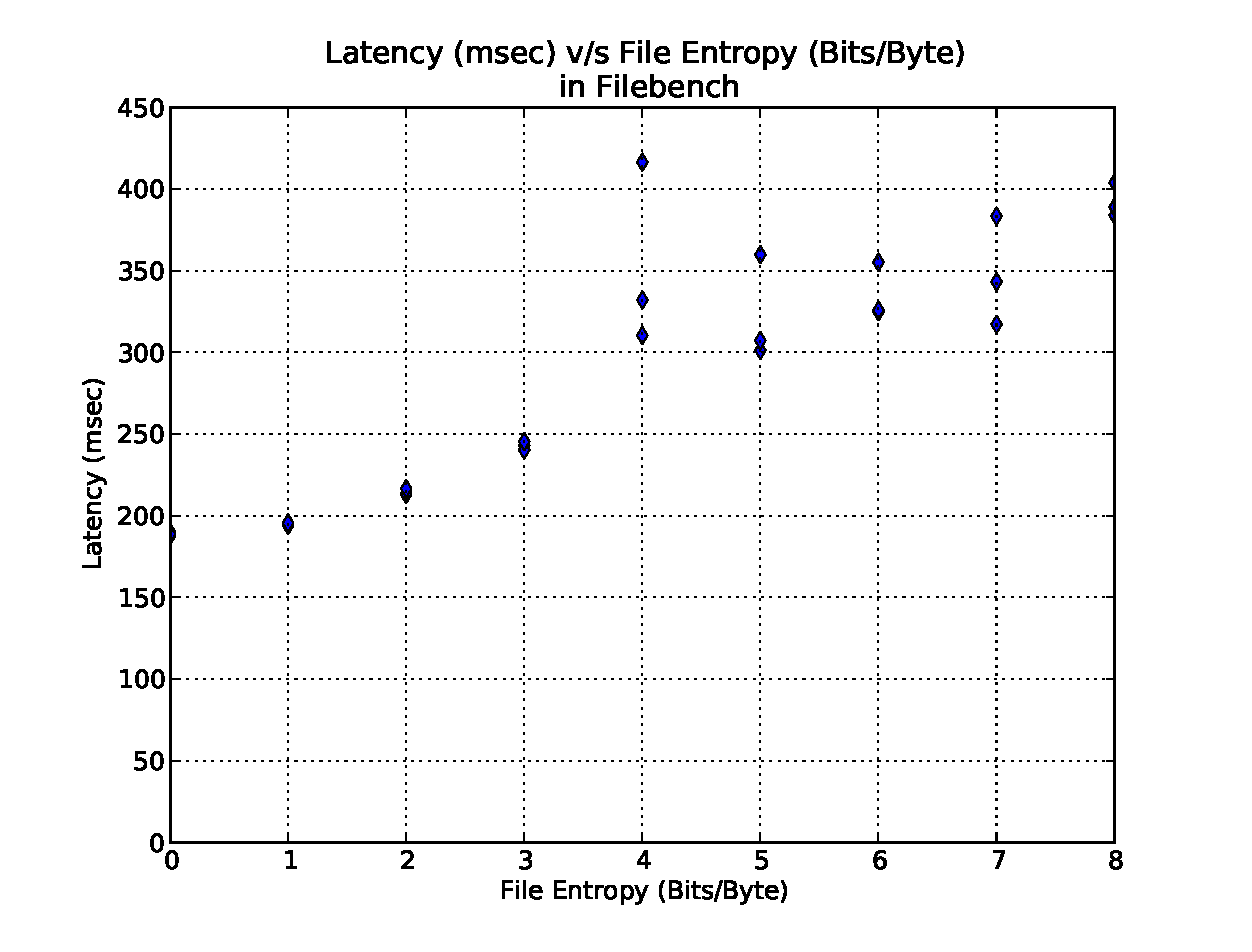
\includegraphics[scale=.55]{../results/set1/write_latency_all.eps}
\caption{The latency of all the different write runs}
\label{fig:wl}
\end{center}
\end{figure}


\begin{figure}[H]
\begin{center}
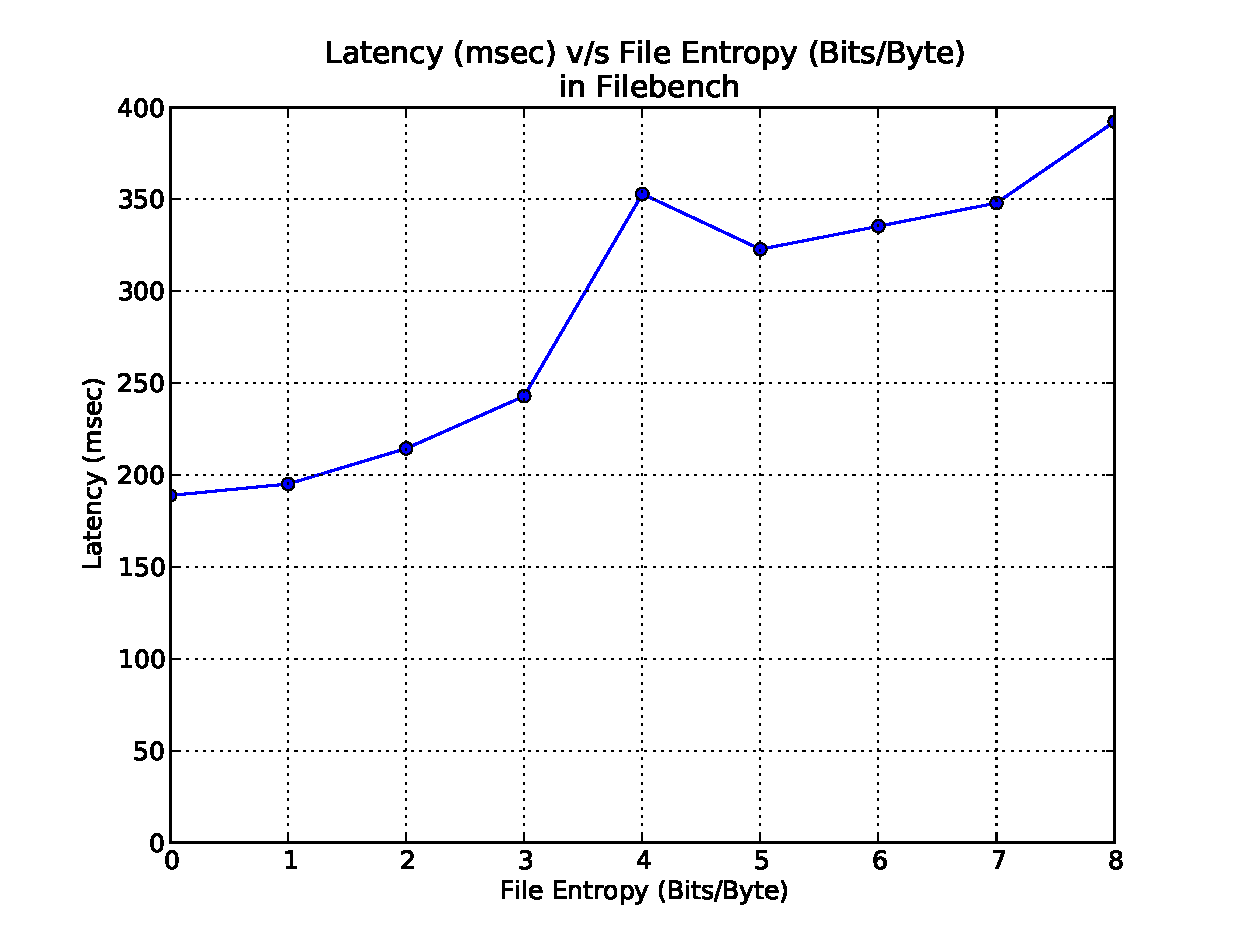
\includegraphics[scale=.55]{../results/set1/write_latency_avg.eps}
\caption{The average latency over all the write runs}
\label{fig:wlavg}
\end{center}
\end{figure}
\paragraph{}
On the other hand, figure \ref{fig:wl} and \ref{fig:wlavg} show that latency of the write operation is increasing as the entropy increased. The larger the entropy the more effort that SDFS spend to deduplicate the files and the larger the latency will be for each write operation. Figure \ref{fig:wl} shows all values of latency collected from 27 runs. The deviation is small and acceptable. To present all the runs on one plot the average of all the runs for each entropy is calculated and presented in figure \ref{fig:wlavg}.

\begin{figure}[H]
\begin{center}
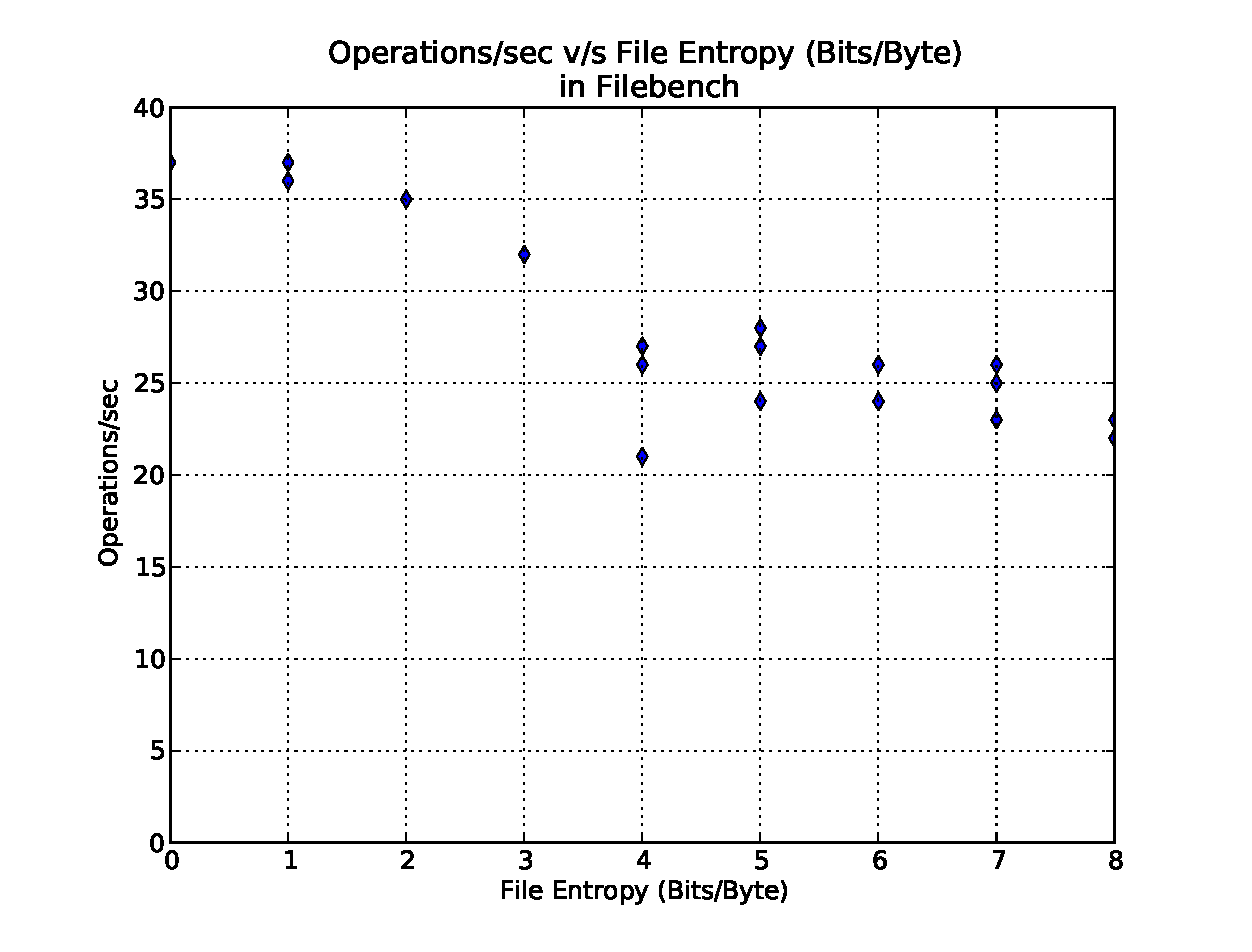
\includegraphics[scale=.55]{../results/set1/write_ops_all.eps}
\caption{The operations execution-speed of all the write runs}
\label{fig:wops}
\end{center}
\end{figure}


\begin{figure}[H]
\begin{center}
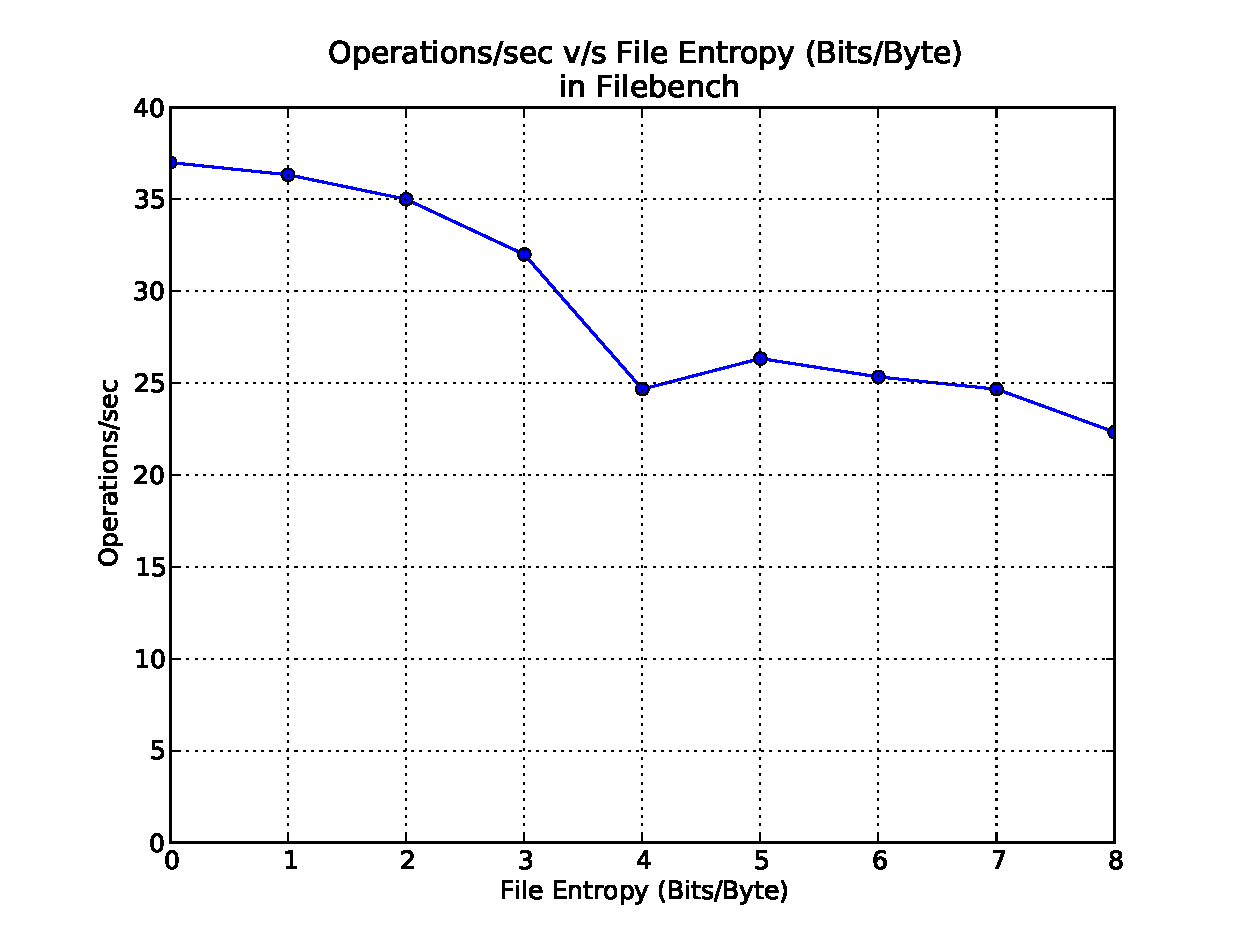
\includegraphics[scale=.55]{../results/set1/write_ops_avg.eps}
\caption{The average operations execution-speed over all the write runs}
\label{fig:wopsavg}
\end{center}
\end{figure}

\paragraph{}
The results depicted by figure \ref{fig:wops} are as expected. Moreover, they show us the effect of ops/sec on bandwidth and latency. The less we operations we can execute per second the less the size of data we can write which decrease the bandwidth.
 In the same manner if we want more time to execute a specific amount of operations, this means that the latency of the write operations is increased. Figure \ref{fig:wopsavg} shows the average of the three readings obtained for each entropy value.

\begin{figure}[H]
\begin{center}
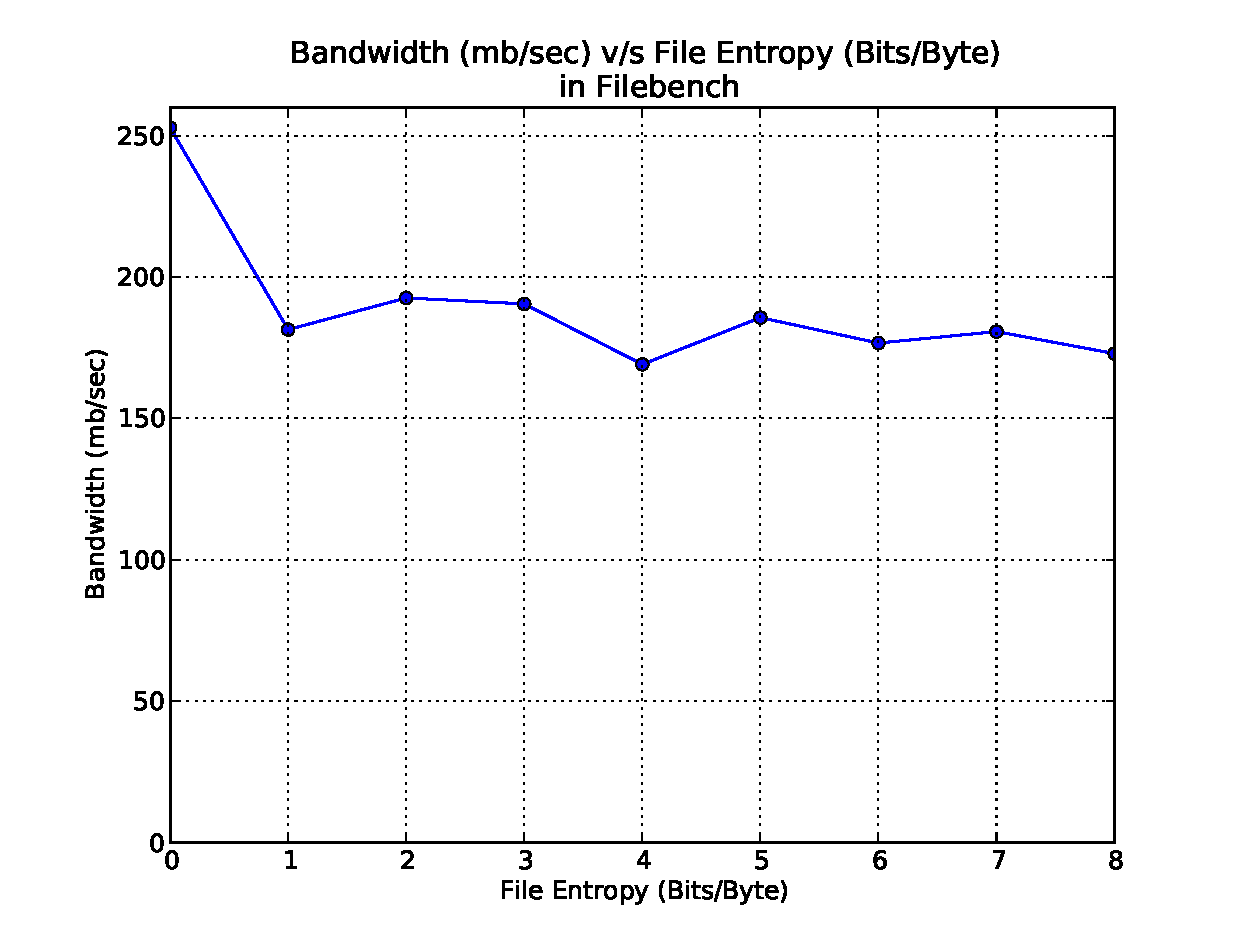
\includegraphics[scale=0.55]{../results/set1/read_bw.eps}
\caption{The bandwidth of all the read runs }
\label{fig:rb}
\end{center}
\end{figure}

\begin{figure}[H]
\begin{center}
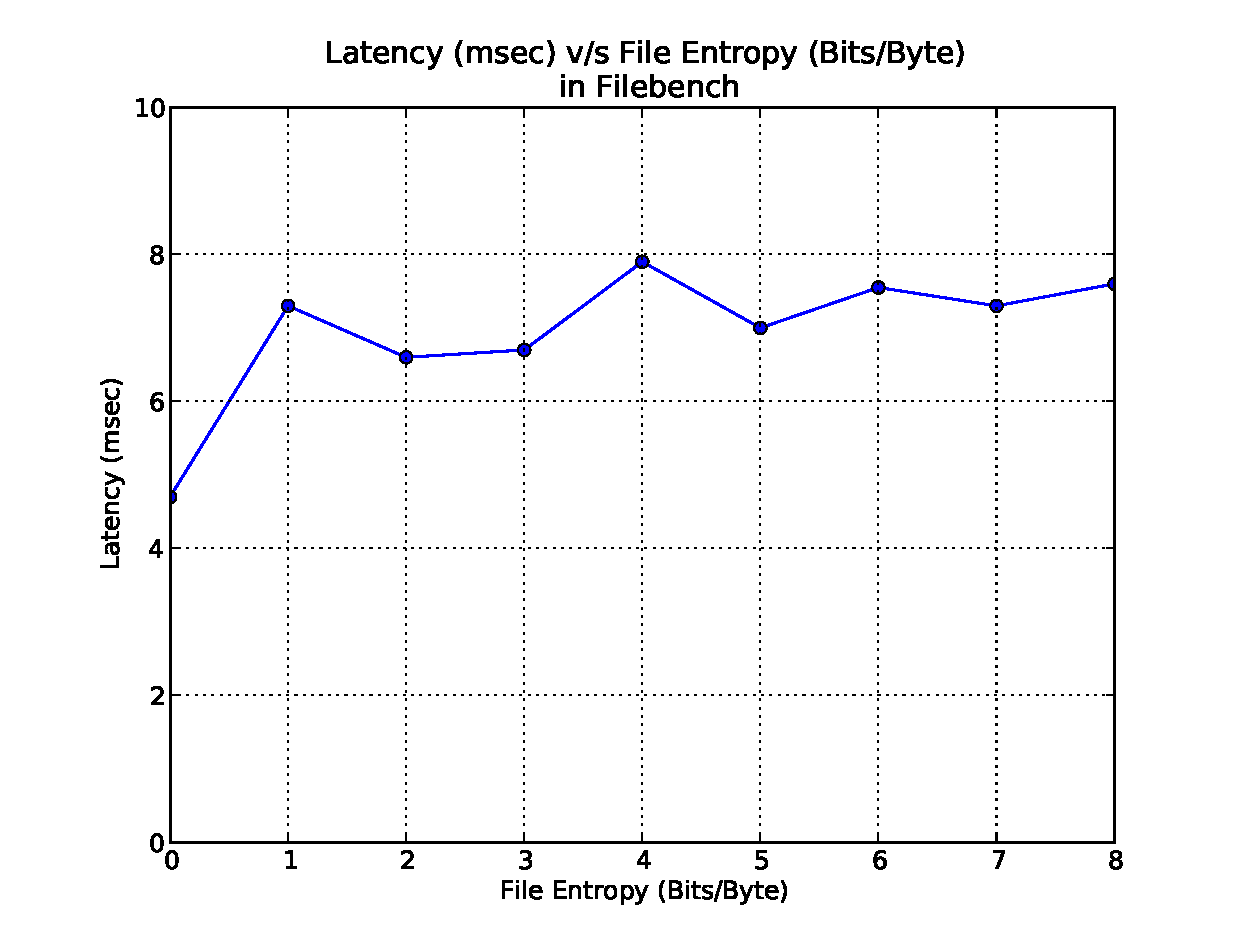
\includegraphics[scale=.55]{../results/set1/read_latency.eps}
\caption{The latency over all the read runs}
\label{fig:rl}
\end{center}
\end{figure}

\paragraph{}
The read workload preallocates around 50 GiB for each run, this takes a lot of time. For this reason we could manage to run more than once. However, figure \ref{fig:rb} and \ref{fig:rl} show clearly that the read workload follow the same behavior of the write workload as the entropy increases.

\section{Lookup fill method results}


The following results were generated by using \verb+entropy_lookup_fill+\footnote{section \ref{sec:ent_imp}} method.

\begin{figure}[H]
\begin{center}
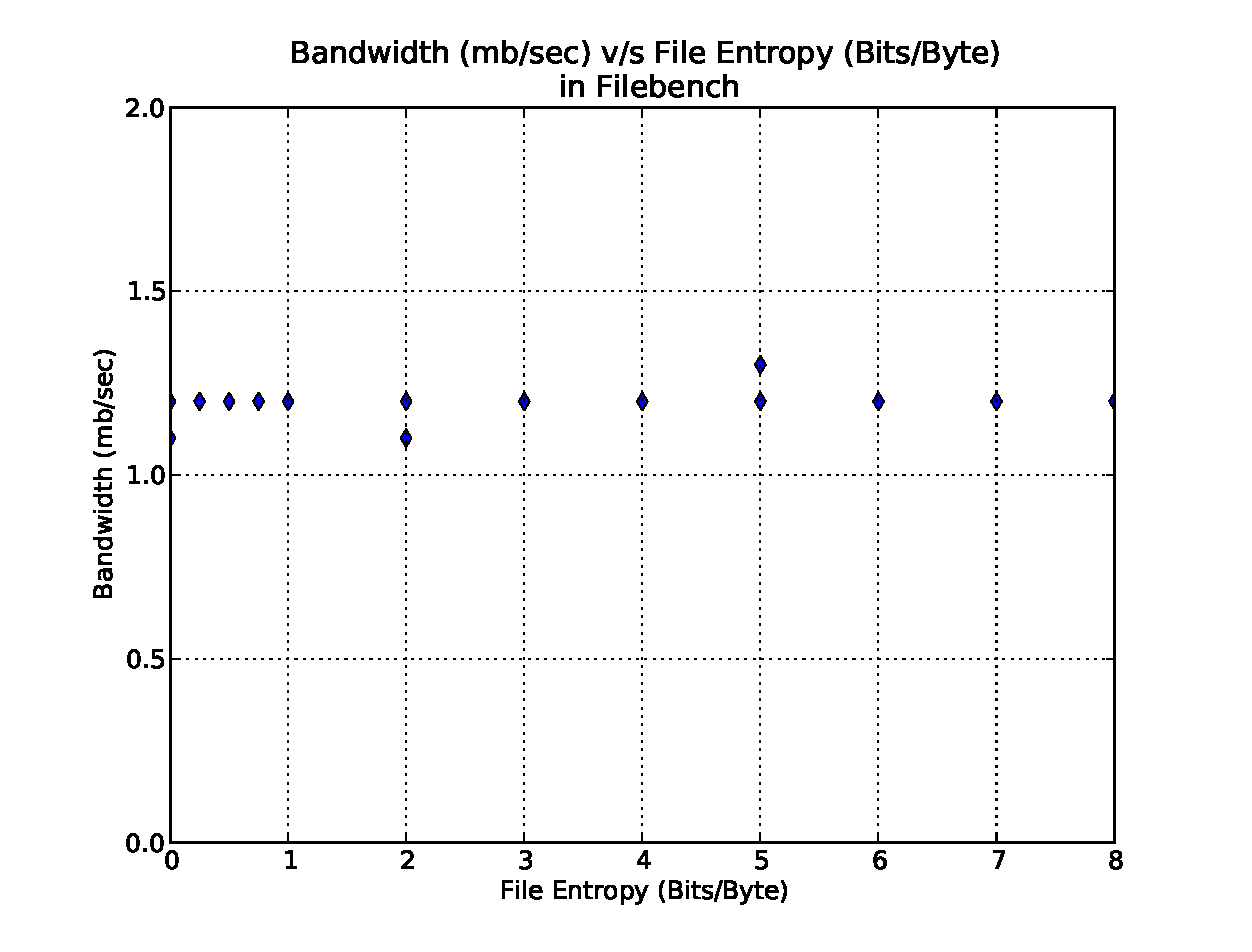
\includegraphics[scale=.55]{../results/set2/write_bw_2.eps}
\caption{The bandwidth of all the write runs}
\label{fig:wb2}
\end{center}
\end{figure}

\begin{figure}[H]
\begin{center}
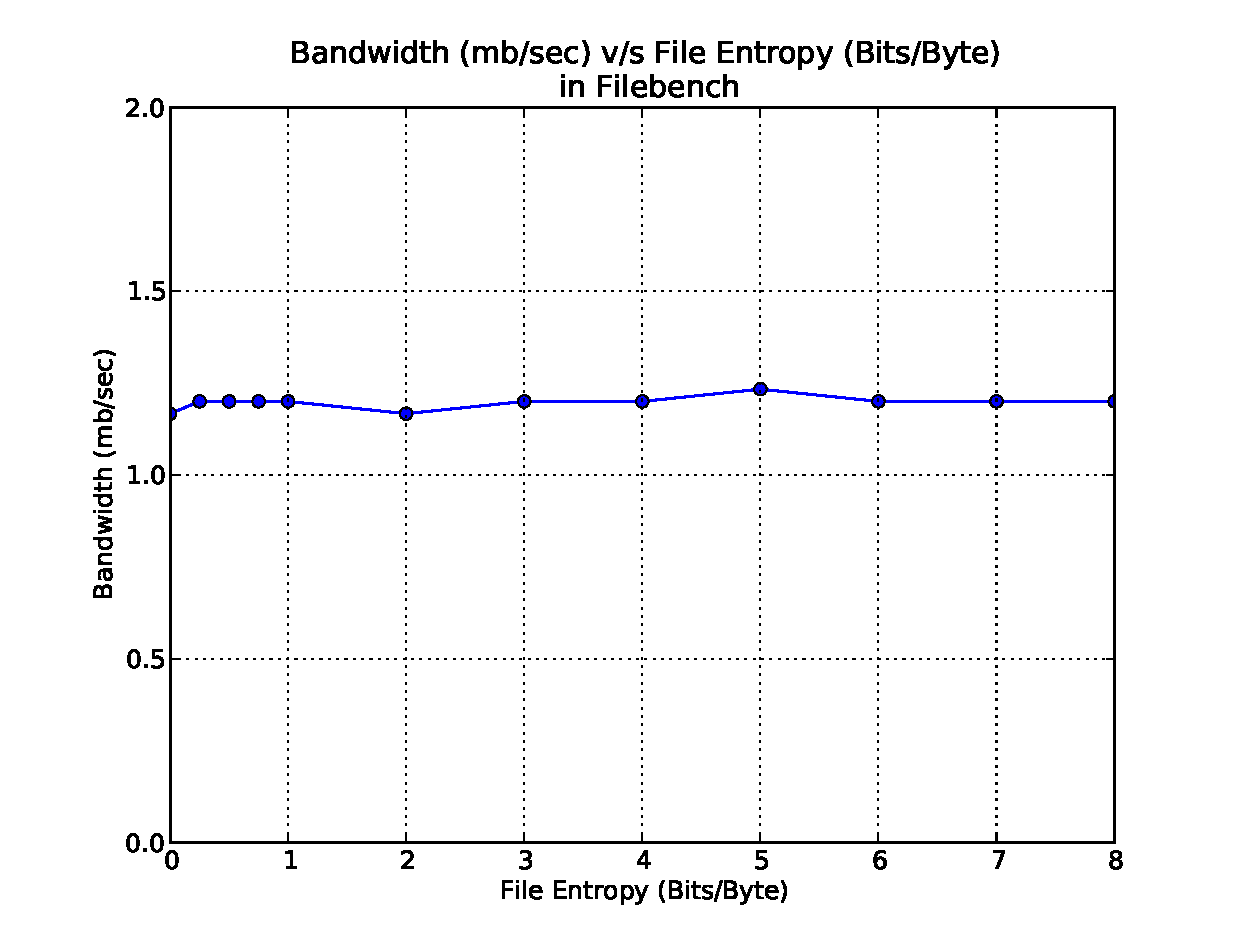
\includegraphics[scale=.55]{../results/set2/write_bw_avg_2.eps}
\caption{The average bandwidth over all the different write runs}
\label{fig:wbavg2}
\end{center}
\end{figure}

Figure \ref{fig:wb2} and \ref{fig:wbavg2} show that the bandwidth of the write operation dropped dramatically to low values compared to the values using \verb+entropy_cont_fill+. The reason behind that, is that the new method takes 3 times the time required by the first method to generate the data which makes the disk idle most of the time, so the average bandwidth achieved is so low. Moreover, the lookup generates random data with homogeneous entropy over the file which makes it so hard for the SDFS to find deplicates chunks in the fileset.

\begin{figure}[H]
\begin{center}
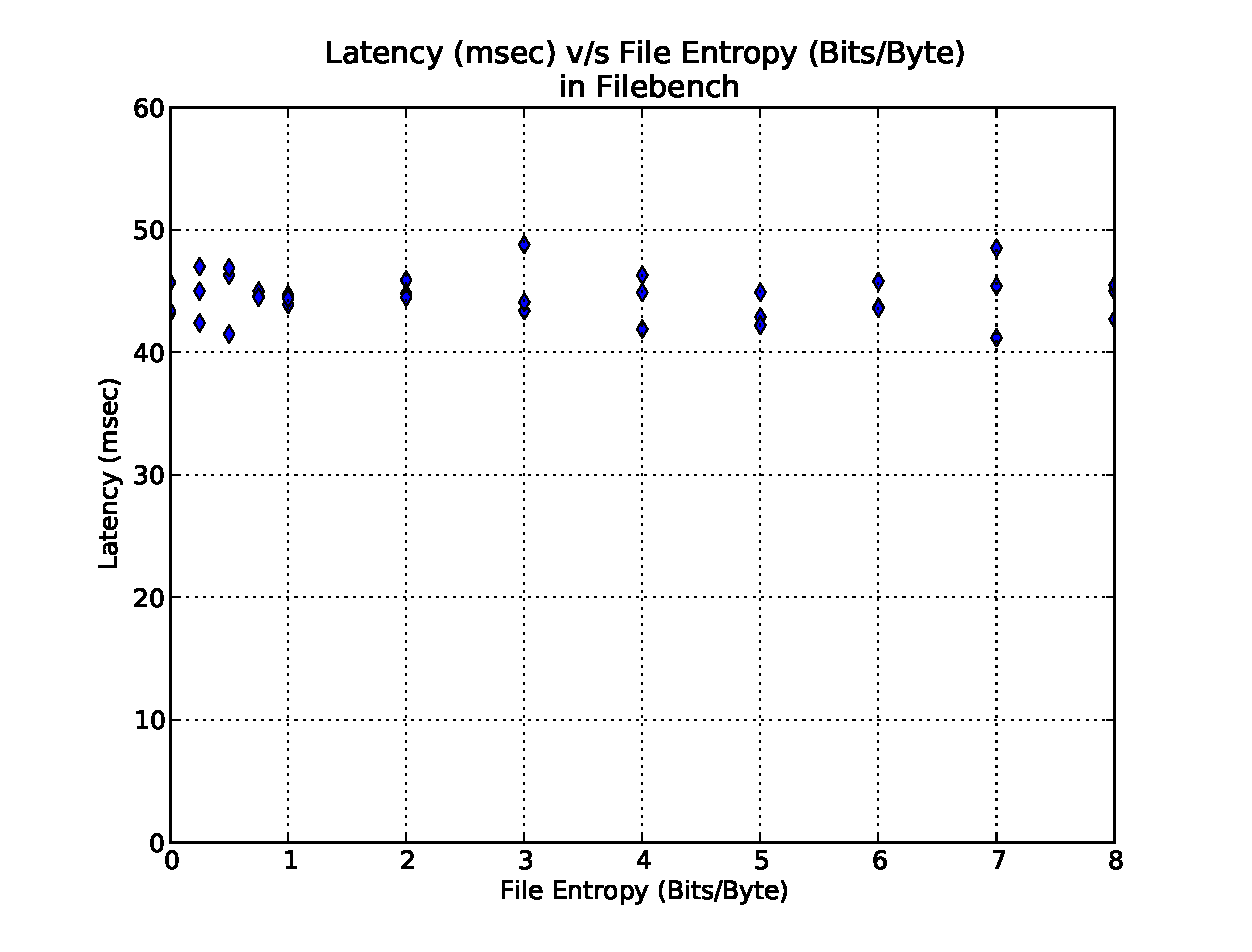
\includegraphics[scale=.55]{../results/set2/write_latency_2.eps}
\caption{The latency of all the different write runs}
\label{fig:wl2}
\end{center}
\end{figure}


\begin{figure}[H]
\begin{center}
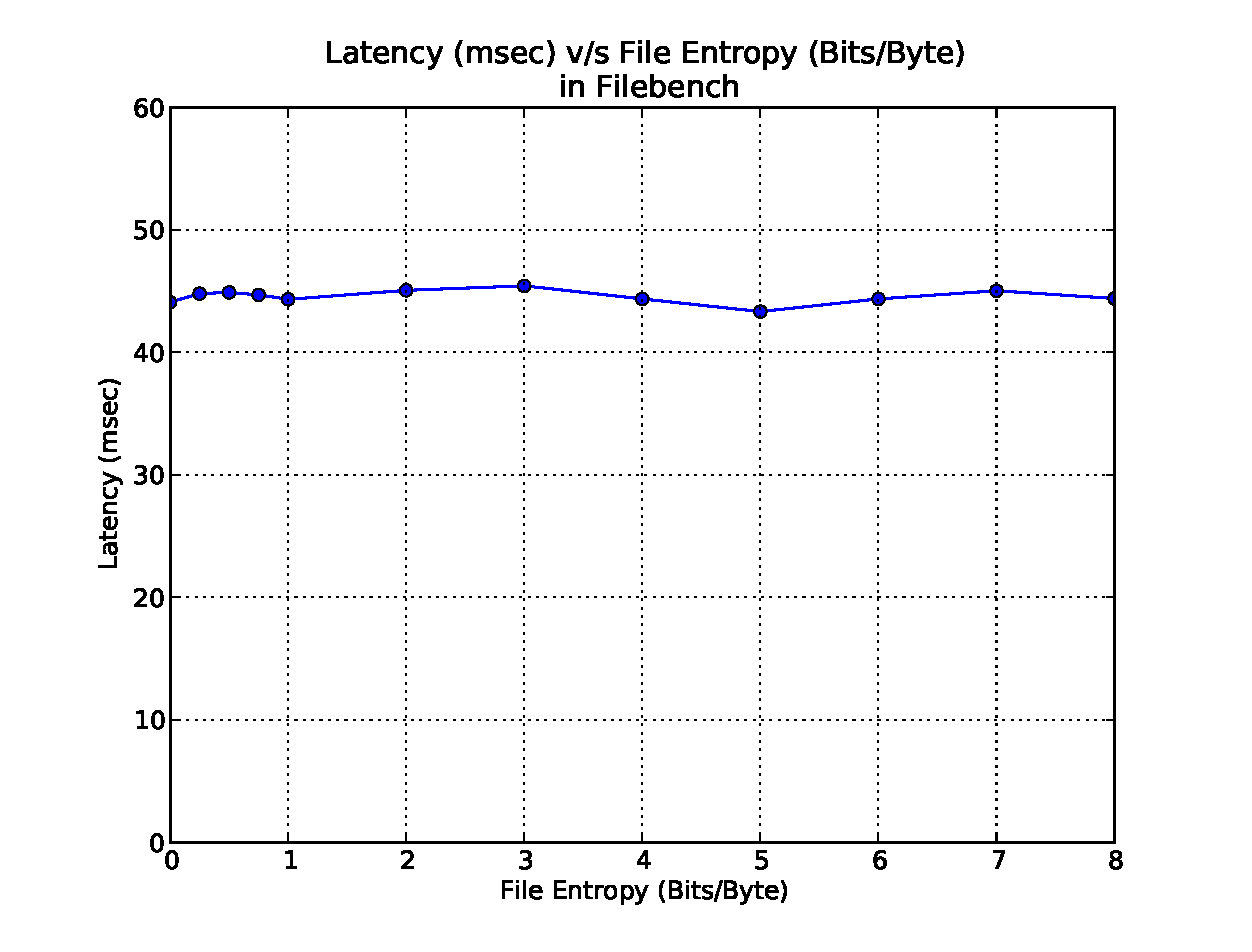
\includegraphics[scale=.55]{../results/set2/write_latency_avg_2.eps}
\caption{The average latency over all the write runs}
\label{fig:wlavg2}
\end{center}
\end{figure}


\begin{figure}[H]
\begin{center}
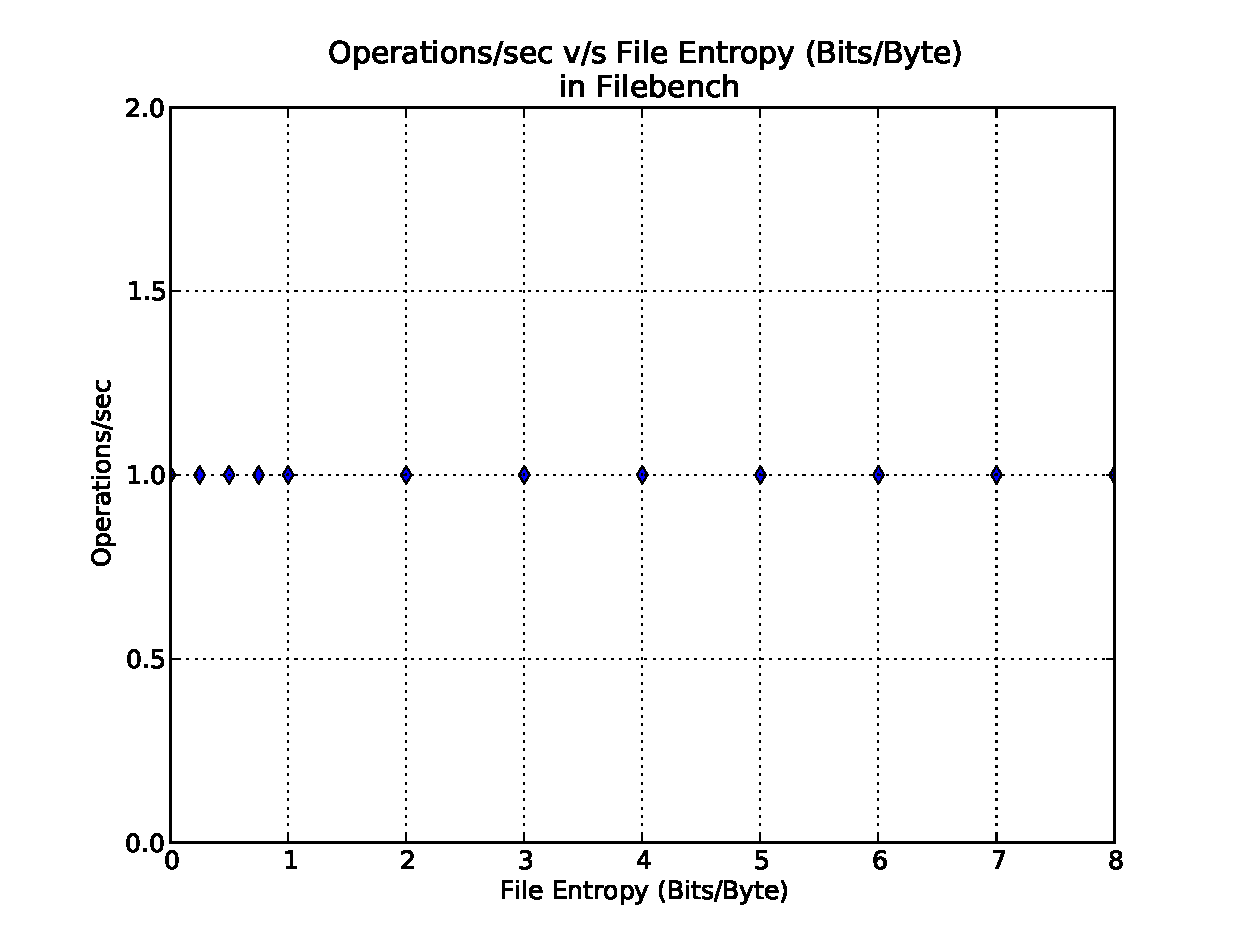
\includegraphics[scale=.55]{../results/set2/write_ops_2.eps}
\caption{The operations execution-speed of all the write runs}
\label{fig:wops2}
\end{center}
\end{figure}


\begin{figure}[H]
\begin{center}
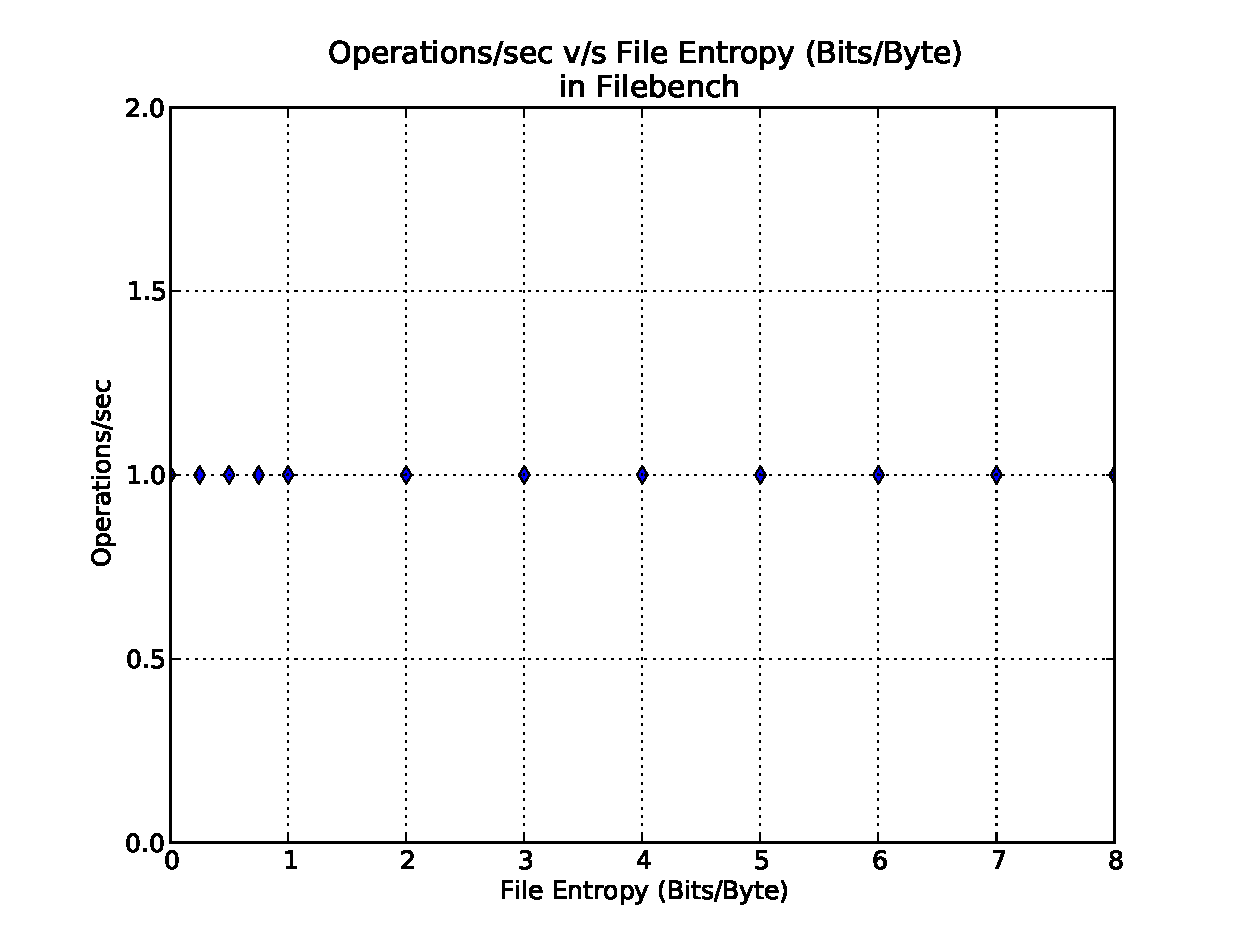
\includegraphics[scale=.55]{../results/set2/write_ops_2.eps}
\caption{The average operations execution-speed over all the write runs}
\label{fig:wopsavg2}
\end{center}
\end{figure}

\begin{figure}[H]
\begin{center}
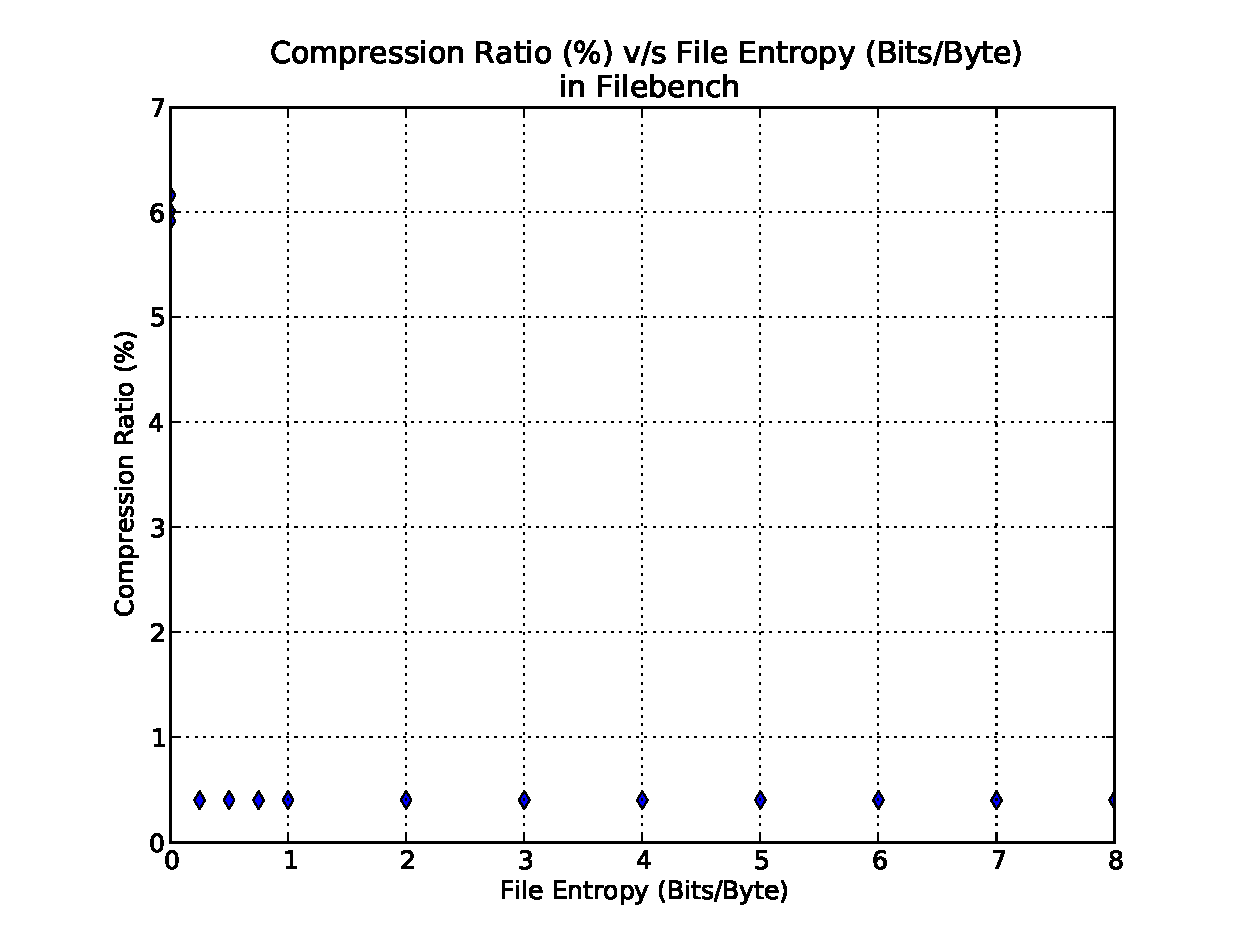
\includegraphics[scale=.55]{../results/set2/write_comp_2.eps}
\caption{The compression ratio of all the write runs}
\label{fig:comp2}
\end{center}
\end{figure}


\begin{figure}[H]
\begin{center}
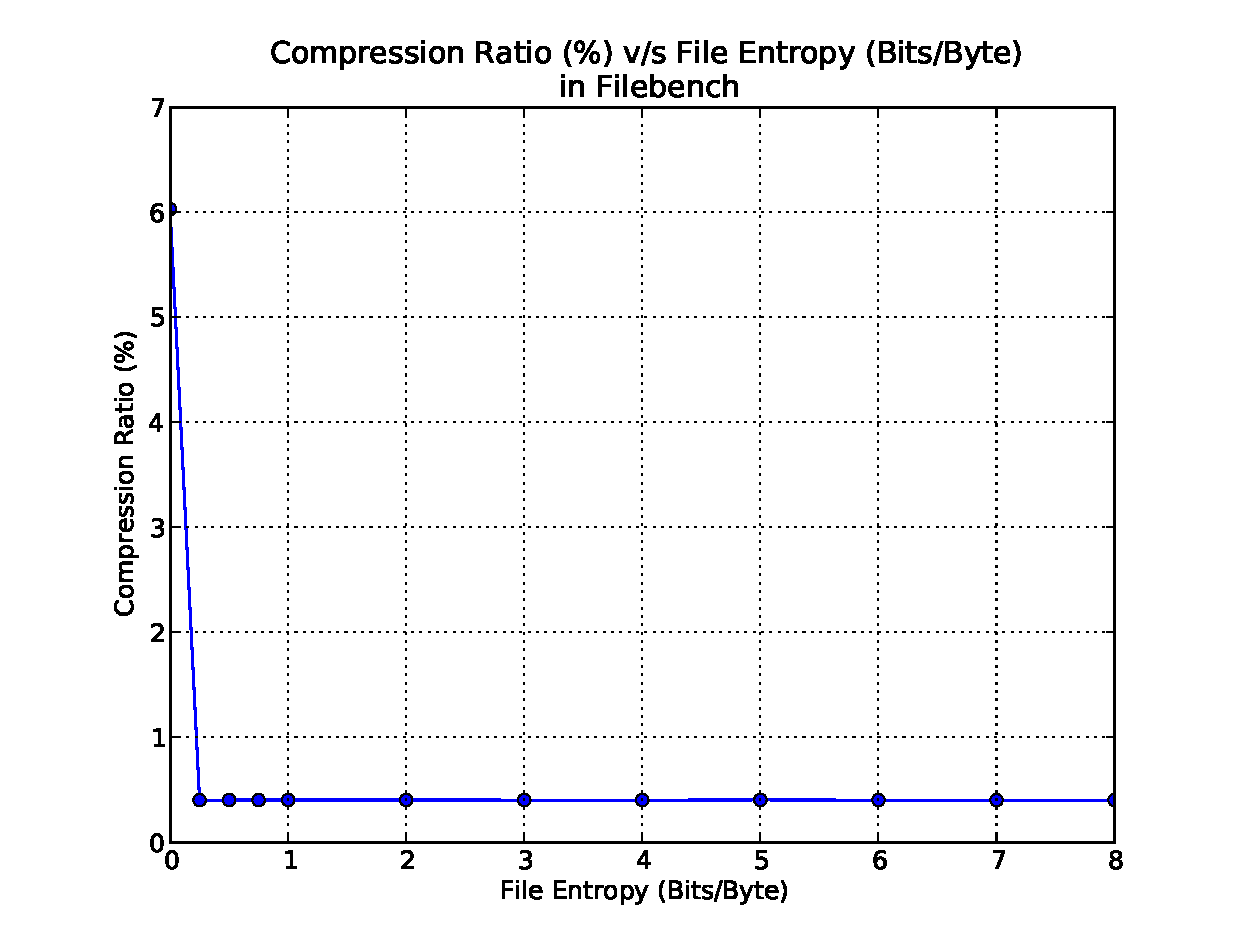
\includegraphics[scale=.55]{../results/set2/write_comp_avg_2.eps}
\caption{The compression ratio average over all the write runs}
\label{fig:compavg2}
\end{center}
\end{figure}

Figure \ref{fig:comp2} and \ref{fig:compavg2}

\chapter{Conclusions}\label{chap:conc}
\chapter{Future Work}\label{chap:fut}


Currently generating the random data takes a lot of time, except for the contiguous method explained in section \ref{sec:ent_imp}.
This makes the processor lags behind the disk, which keeps the disk idle most of the time.
 However, this should not affect the results when we compare the readings obtained from different levels of an entropy used with a deduplication file system.
 However, testing other non-deduplication filesystems with entropy generation enabled will cause unexpected results because of the way the statistics are collected in Filebench.
\paragraph{}
 Filebench calculates the averages bandwidth and operations per second.
 Therefore, if the entropy is enabled while running filebench on ext2 for example, most of the time the disk will be idle which will result in lower readings than the case if entropy is switched off, although ext2 is not aware of the data that is being written the previous scenario 
\paragraph{}
To fix this, Filebench has to be modified to calculate the time the disk is actually used and use only that time to calculate the average bandwidth and operations per second.
\paragraph{}
Another point to mention is the model we are using to model practical loads. We are using entropy as the only characteristics of the file that is actually varied.
 Moreover, it is the same value across all the files. In normal loads like the ones in cloud computing servers where there is a lot of backups and snapshots, the entropy can high per file but the redundancy is also high.
 Using true randomization makes it so hard to generate any chunk of the file twice.
 Maybe it is better to generate a more realistic model by profiling large amount of storage and construct the PDF from that data. We can use such PDF to to calculate the probability that a page will be redundant to one already have been written on the disk.
